\documentclass{article}
\usepackage{booktabs}
\usepackage{amsmath}
\usepackage{graphicx}
\usepackage{caption}
\usepackage{listings}
\usepackage{xcolor}
\usepackage{pxfonts}
\lstset{
  basicstyle=\ttfamily,
  columns=fullflexible,
  breaklines=true,
  postbreak=\raisebox{0ex}[0ex][0ex]{\color{red}$\hookrightarrow$\space}
} 
\title{Homework}
\author{Zhijiia Chen}
\begin{document}

\section{HW3}

\paragraph{1.} Assign a letter to each node as shown in Fig.~\ref{fig:topo}.
\begin{figure}
    \centering
    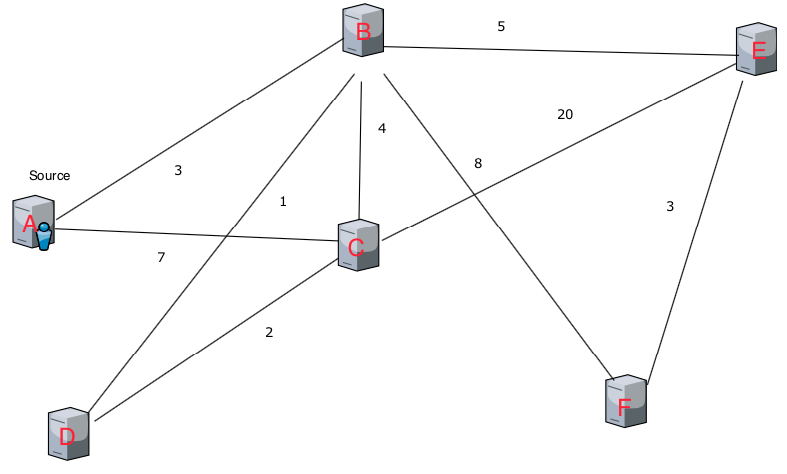
\includegraphics[width=\linewidth]{fig/topo.png}
    \caption{network topology
    } \label{fig:topo}
\end{figure}
Define the following notation:

\begin{itemize}
    \item $d(v)$: cost of the least-cost path from the source node to destination $v$ as of this iteration of the algorithm.
    \item $d_x(y)$ current minimum cost from node x to node y.
    \item $c(x, y)$ cost from x to directly attached neighbor y.
    \item $p(v)$: previous node (neighbor of $v$) along the current least-cost path from the source to $v$.
    \item $N$: all the nodes.
    \item $N'$: subset of nodes; $v$ is in $N'$ if the least-cost path from the source to $v$ is definitively known.
\end{itemize}

\textbf{Link-State (Dijkstra algorithm)}: 

\begin{lstlisting}[mathescape=true]
    N' = {A}
    for all nodes v
        if v is a neighbor of A then
            d(v) = c(A, v)
        else 
            d(v) = $\infty$
    loop
        find w not in N' such that d(w) is a minimum
        add w to N'
        update d(V) for each neighbor v of w and not in N':
            d(v) = min(d(v), d(w) + c(w, v))
    until N' = N
\end{lstlisting}

Table~\ref{tab:dijkstra} shows all the rounds using Dijkstra algorithm to find the shortest paths. In the table, \textbf{N'} is a set contains the nodes whose shortest path costs are already known. Each row in the table is a round that computes the shortest path cost from the sourcce noede (A) to a picked node. For cells in the columns titled with nodes letters, '-' means we already know the least cost to the node. Value (X, y) means current path cost from source node A to the node (denoted by the column title) is y, and the previous node is X. For example, in the first row of column F, "A, $\infty$" means current path cost to node F is infinte (unknown), and in the third row of column C, "D, 6" means current path cost to node C is 6 and the previous node is node D.

\begin{table}[h!]
    \begin{center}
      \caption{Find shortest path using Dijkstra algorithm.}
      \label{tab:dijkstra}
      \begin{tabular}{c|c|c|c|c|c|c|c} % <-- Alignments: 1st column left, 2nd middle and 3rd right, with vertical lines in between
        \toprule
        \textbf{Picked node}& \textbf{N'}& \textbf{A}&\textbf{B}&\textbf{C}&\textbf{D}&\textbf{E}&\textbf{F}\\
        \hline
        A&\{A\}&-&A, 3&A, 7&A, $\infty$&A, $\infty$&A, $\infty$\\
        \hline
        B&\{A, B\}&&-&A, 7&B, 4&B, 8&B, 11\\
        \hline
        D&\{A, B, D\}&&&D, 6&-&B, 8&B, 11\\
        \hline
        C&\{A, B, C, D\}&&&-&&B, 8&B, 11\\
        \hline
        E&\{A, B, C, D, E\}&&&&&-&B, 11\\
        \hline
        F&\{A, B, C, D, E, F\}&&&&&&-\\
        \bottomrule
      \end{tabular}
    \end{center}
  \end{table}

According to the table, we can get the shortest path from A to all other nodes:

From A to B: A-$>$B, cost = 3.

From A to C: A-$>$B-$>$D-$>$C, cost = 6.

From A to D: A-$>$B-$>$D, cost = 4.

From A to E: A-$>$B-$>$E, cost = 8.

From A to F: A-$>$B-$>$F, cost = 11.
\end{document}
